\section{Blueboat}

À défaut d'avoir des AUV à disposition, il a été décidé avec nos encadrants d'utiliser des blueboats pour réaliser notre projet. Cette partie vise à présenter ces robots, expliquer leur fonctionnement, et permettre à de futurs élèves ou personnels d'apprendre à les connaître et de les prendre en main facilement.

\subsection{Présentation}

Les BlueBoats (voir Figure \ref{fig:blueboat}) sont des USV développés par la société Blue Robotics \cite{bluerobotics_site}. Ces robots sont des bicoques équipés de deux propulseurs, d'un routeur Wi-Fi, d'une carte Raspberry Pi 4 couplée à une carte Navigator, et de divers capteurs, les deux plus notables étant un GPS et une IMU. Ces robots ont l'avantage d'offrir un bon rapport qualité-prix et d'être particulièrement modulable, les rendant adaptés à une large gamme de missions.
Les BlueBoats disposent de leur propre OS BlueOS. Ce dernier permet de paramétrer simplement le robot, de communiquer avec lui via le protocole Mavlink, de le contrôler via un firmware comme Ardupilot, mais aussi d'installer certaines librairies utiles comme des applications pour utiliser certains capteurs ou des interfaces ROS/Mavros offrant d'autres solutions que le passage par MavLink pour contrôler le bateau. L'utilisation de firmware comme Ardupilot permet aussi de contrôler le robot directement sur son ordinateur grâce à des logiciels tels que QGround Control ou MissionPlanner. La Figure \ref{fig:archi_blueboat} présente de façon simplifiée les différentes composantes logicielles liées au BlueBoat et leurs interactions.
Afin de se connecter facilement aux BlueBoats où que l'ont soit, BlueRobotics vend aussi des "Base Station" (voir Figure \ref{fig:base_station}), qui sont des boîtiers équipés d'une antenne amovible permettant de créer un réseau WiFi local. Pour obtenir une portée plus importante, l'antenne de la Base Station peut être remplacée par une antenne directionnelle vendue sur le site de BlueRobotics.

\begin{figure}[h]
        \centering
        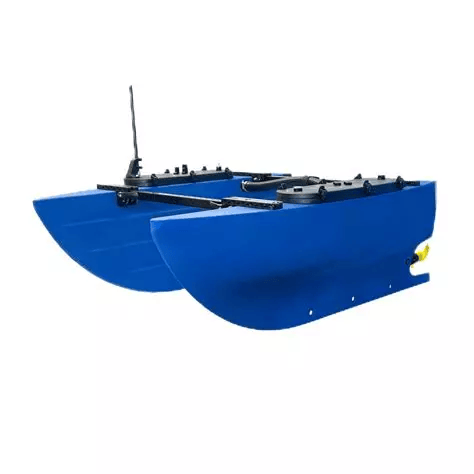
\includegraphics[width=0.5\linewidth]{images/blueboat.png}
        \caption{BlueBoat}
        \label{fig:blueboat}
    \end{figure}

\begin{figure}[h]
        \centering
        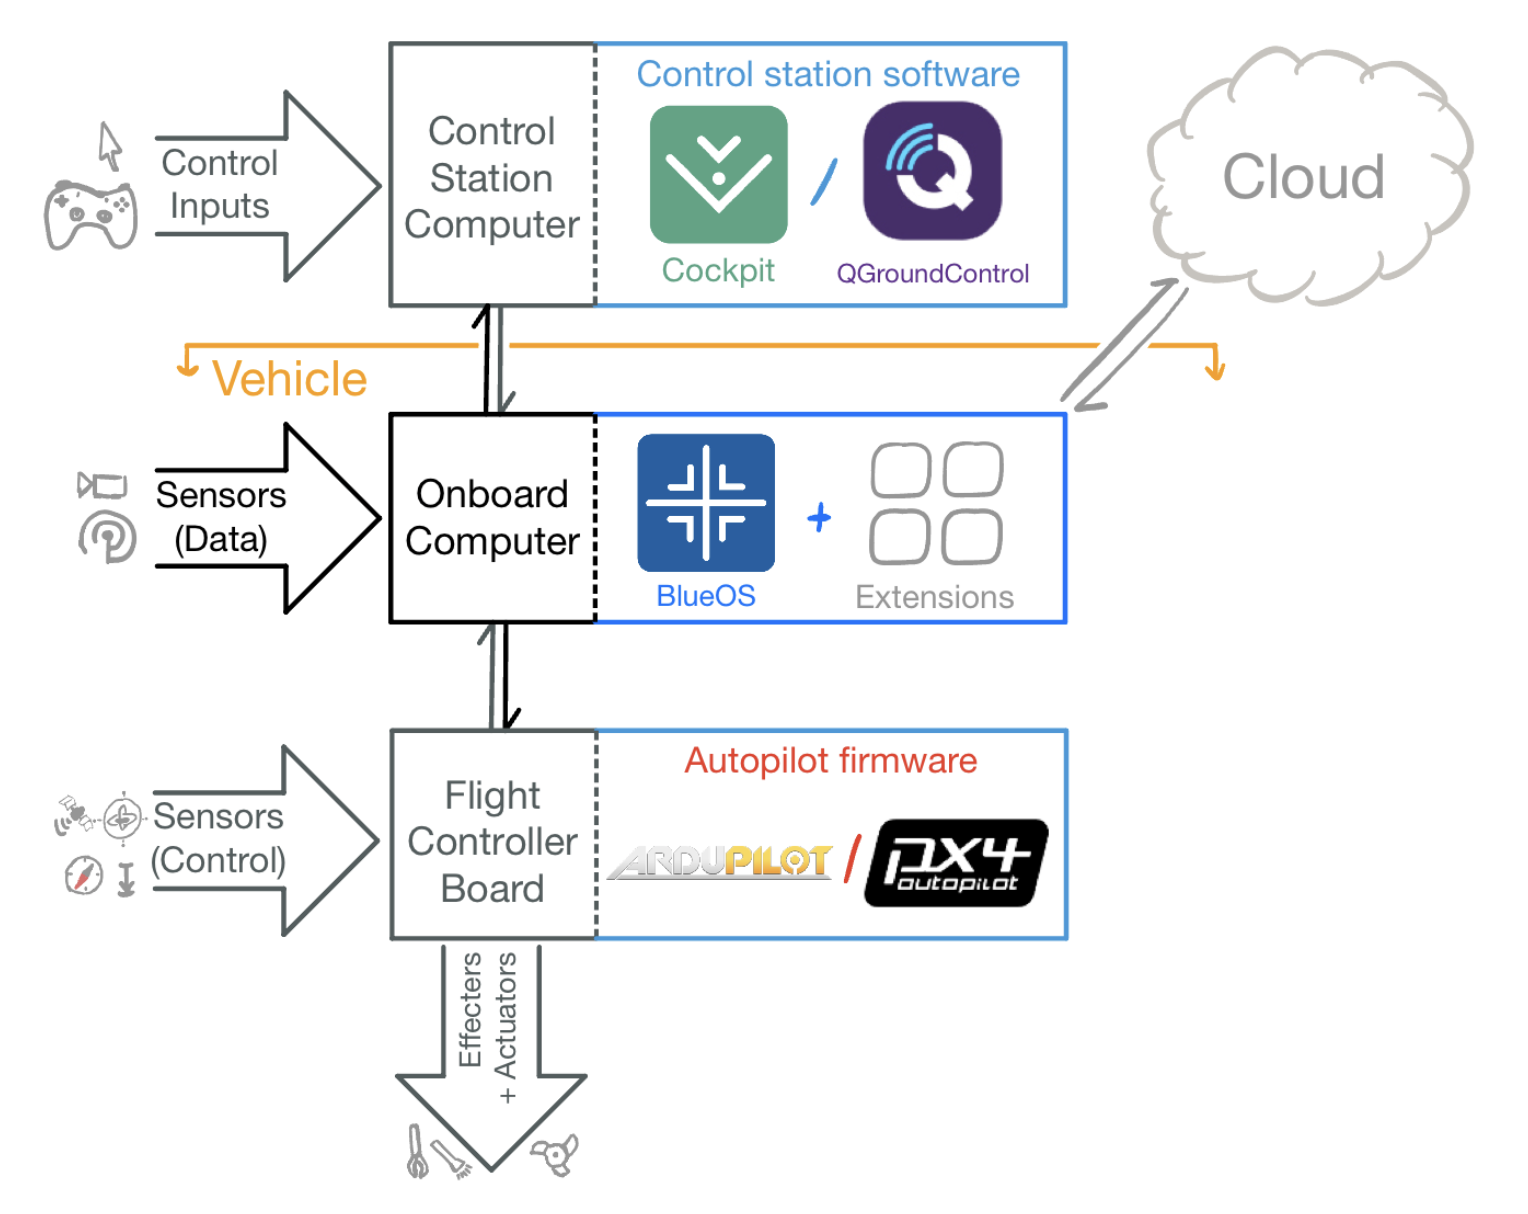
\includegraphics[width=0.8\linewidth]{images/archi.png}
        \caption{Architecture logicielle simplifiée du BlueBoat présentée sur le site dédié à BlueOS\footnote{\url{https://blueos.cloud/docs/latest/usage/overview/}}}
        \label{fig:archi_blueboat}
    \end{figure}

\begin{figure}[h]
        \centering
        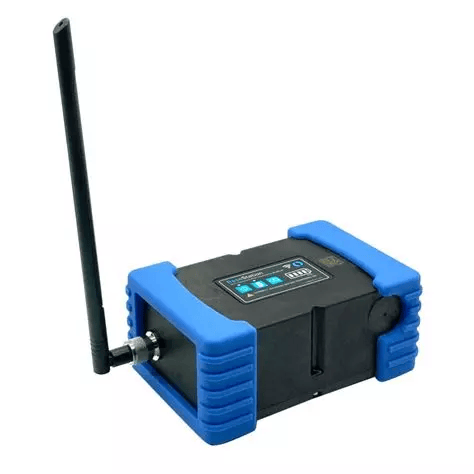
\includegraphics[width=0.5\linewidth]{images/base_station.png}
        \caption{Base Station}
        \label{fig:base_station}
    \end{figure}

\subsection{Prise en main}

    Les instructions pour prendre en main les robots sont disponibles sur le site de Blue Robotics \cite{blueboat_docs}. Elles consistent globalement dans l'ordre en le paramétrage de la Base Station, puis celui du routeur WiFi du BlueBoat et enfin de BlueOS. Il nous a été demandé de respecter quelques conventions propres à l'ENSTA et différentes de celles porposées par Blue Robotics concernant les adresses IP des différents composants sur le réseau de la Base Station, mais cela a peu d'impact sur la procédure de prise en main des robots. Les conventions propres à l'ENSTA sont décrites par le tableau \ref{tab:ip_plan_blueboat}.

    \begin{table}[h]
        \centering
        \caption{Plan d'adressage utilisé pour la flotte BlueBoat.}
        \label{tab:ip_plan_blueboat}
        \renewcommand{\arraystretch}{1.3}
        \begin{tabular}{p{0.34\linewidth} p{0.56\linewidth}}
            \toprule
            \textbf{Composant} & \textbf{Adresse IP par défaut}& \textbf{Adresse IP ENSTA} \\
            \midrule
            Ordinateur de contrôle & \texttt{192.168.2.1} & \texttt{192.168.2.11X} \\
            Raspberry Pi BlueBoat $X$ & \texttt{192.168.2.2} & \texttt{192.168.2.20X} \\
            Base Station & \texttt{192.168.2.3} & \texttt{192.168.2.1} \\
            Routeur WiFi BlueBoat $X$ & \texttt{192.168.2.4} & \texttt{192.168.2.10X} \\
            \bottomrule
        \end{tabular}
    \end{table}


    Dans notre cas, puisque nous utilisons plusieurs robots à la fois, il faut changer les identifiants des robots dans le réseau MavLink via le paramètre SYSID_THISMAV. Pour contrôler les robots directement via MavLink, il est aussi nécessaire d'ajouter l'adresse IP et le port de notre ordinateur à la liste des \textit{MavLink endpoints} (accessible via le "mode pirate" de BlueOS) en tant que "Client UDP", soit en modifiant l'endpoint \textit{GCS Client Link}, soit en en créant un nouveau.

    Afin de pouvoir reprendre le contrôle manuel du BlueBoat même en cas de perte de connexion à la Base Station, il a été décidé d'installer sur ceux-ci des récepteur \textit{TBS CrossFire} liés à des émetteurs branchés à des télécommandes \textis{FrSky Taranis QX7}. Il était déjà possible, via QGroundControl, de contrôler les robots avec des joysticks connectés à l'ordinateur mais cette solution offrait une portée moindre. L'ajout d'une télécommande aux Blueboats ne nécessite pas d'ajout de lignes de codes ou l'installation d'une extension particulière sur BlueOS mais simplement le changement de certains paramètres, en particulier les paramètres RCX_FUNCTION qui attribue à chaque channel RC un rôle, tel que prendre la priorité sur les commandes moteur ("RC_OVERRIDE_ON"), armer ou désarmer les moteurs, changer le mode de contrôle du robot, contrôler la poussée ou la rotation, etc. Les paramètres choisis dans notre cas sont présenté par le tableau \ref{tab:param_telecom}. Il faut aussi paramétrer les boutons de la télécommandes pour les associer aux canaux correspondants.

    \begin{table}[h]
        \centering
        \caption{Paramètres modifiés pour utiliser les télécommandes sur les BlueBoats}
        \label{tab:param_telecom}
        \renewcommand{\arraystretch}{1.2}
        \begin{tabular}{p{0.34\linewidth} p{0.56\linewidth}}
            \toprule
            \textbf{Paramètre} & \textbf{Valeur} \\
            \midrule
            RC6_OPTION & \texttt{ArmDisarm (4.2 and higher)} \\
            RC10_OPTION & \texttt{RC Override Enable} \\
            RCMAP_ROLL & \texttt{1} \\
            RCMAP_PITCH & \texttt{2} \\
            RCMAP_THROTTLE & \texttt{3} \\
            RCMAP_YAW & \texttt{4} \\
            MODE_CH & \texttt{5} \\
            MODE1 & \texttt{Manual} \\
            MODE2 & \texttt{Manual} \\
            MODE3 & \texttt{Hold} \\
            MODE4 & \texttt{Hold} \\
            MODE5 & \texttt{Guided} \\
            MODE6 & \texttt{Guided} \\
            \bottomrule
        \end{tabular}
    \end{table}

\subsection{Observations sur le comportement des BlueBoats}

    Les test des BlueBoats, que ce soit via des algorithmes ou un contrôle à la télécommande, ont mis en lumière les difficultés à contrôler le robot. En effet, si la commande envoyée au robot correspond à un changement de direction pur (exemple : commande de + X à droite et -X à gauche), le mouvement du robot ne correspondra lui pas à une rotation pure, mais à une rotation accompagnée d'une vitesse vers l'avant. Il semble possible d'effectuer une rotation pure en donnant en plus au robot une commande vers l'arrière, mais nous n'avons pas déterminé si cette commande était constante ou dépendait de la rotation demandée. 
    Une calibration de l'IMU est aussi nécessaire avant d'utiliser le robot. Cette dernière peut se faire via QGC, en calibrant dans un premier lieu l'accéléromètre en mettant le robot dans des positions particulières, puis le magnétomètre en lui faisant effectuer des mouvements aléatoires dans toues les directions.

\subsection{Autres remarques et conseils}

    Il est possible d'utiliser ROS et MAVROS 1 ou 2 pour contrôler les BlueBoats, et ce grâce à des extensions disponibles sur BlueOS. L'extension ROS a été crée par BlueRobotics et est disponible quelle que soit la version de l'OS tant que cette dernière est suffisament récente. Cependant, l'extension ROS2 est elle compatible uniquement avec la version 64 bits de BlueOS (la version par défaut étant une version 32 bits). La dernière version 64 bits de Blue OS au moment de l'écriture de ces lignes (28/02/2026) est accessible via ce lien : \url{https://github.com/bluerobotics/BlueOS/releases/download/1.5.0-beta.20/BlueOS-raspberry-linux-arm64-v8-bookworm-pi5.zip}\footnote{\url{https://blueos.cloud/docs/stable/usage/installation/} propose les dernières versions 32 et 64 bits de BlueOS. Bien que le nom du fichier comporte "pi5", cette version de l'OS est bien compatible avec une Raspberry Pi 4, ou tout du moins les modèles de Raspberry Pi 4 présent par défaut dans les BlueBoats.}. Il suffit pour l'installer d'extraire le fichier .img contenu dans le fichier zip et de le flasher sur une carte microSD à l'aide par exemple de Raspberry Pi Imager\footnote{\url{https://www.raspberrypi.com/software/}} ou de Balena Etcher\footnote{\url{https://www.balena.io/etcher/}}. L'installation de l'extension ROS2 peut alors théoriquement se faire directement sur la nouvelle version de BlueOS 64bits, mais il a été constaté que BlueOS imposait un timeout de 120s sur les téléchargements et installations, et ROS2 étant assez lourd et donc long à télécherger et installer, il n'a donc pas été possible pour nous de l'installer de cette manière. Il est cependant possible d'installer manuellement l'extension via le terminal sur la Raspberry PI en suivant les instructions données dur le Github de l'extension \cite{github_ros2}.

    Avant la mise à l'eau des BlueBoats, il est aussi conseillé d'appliquer le protocole suivant pour limiter les risques une fois le bateau à l'eau : 

    \begin{itemize}
        \item L'IMU du robot est bien calibrée
        \item En activant le RC Override sur la télécommande, on reprend bien le contrôle du robot
        \item L'arrêt du programme, qu'il soit dû à la fin de la tâche visée où à une interruption clavier de l'utilisateur, arrête bien les deux moteurs
        \item La déconnection du robot de la Base Station (simulable facilement en éteignant la BaseStation) entraîne bien après quelques secondes l'arrêt des moteurs \footnote{Si ce n'est pas le cas, s'assurer que le paramètre \textit{FS_GCS_ENABLE} vale bien \textit{Enabled} et \textit{FS_ACTION} vale \textit{Hold}. Vérifier aussi la valeur de \textit{FS_GCS_TIMEOUT}.}
        \item Après une déconnexion de la Base Station ayant entraîné un arrêt du robot, il est bien possible de reprendre le contrôle via la télécommande (cela nécessite normalement de remettre le mode de contrôle du robot sur "\textit{Manual}", d'où le choix des paramètres pour notre télécommande.)
    \end{itemize}

\subsection{Simulation Ardurover}

    Entre la première et la deuxième campagne de tests à Guerlédan, nous avons souhaité tester une simulation plus réaliste que celles que nous avions déjà réalisée avec Python pour tester nos algorithmes de localisation. Notamment, nous souhaitions obtenir une simulation de robot controlable de la même façon que les BlueBoat, et avec une cinématique plus proche de la réalité. Mr. Lebars nous a fournit une solution potentielle pour y parvenir sous la forme du document \cite{lebars_simu}. Ardurover permet en effet de créer une simulation de drone de surface que l'on peut contrôler via MavLink ou ROS de la même manière qu'un vrai BlueBoat, ainsi que le connecter via TCP à GQC ou d'autres logiciels similaires pour pouvoir visualiser l'état du robot. Cela nécessite une configuration préccise, chaque bateau simulé devant communiquer en TCP avec plusieurs programmes sur des ports différents tels que MavRos, QGC, etc. Utiliser plusieurs bateaux simulés à la fois demande aussi de s'assurer que chaque robot dispose de ses propres ports TCP, noeuds ROS, identifiants mavlink, etc. La configuration requise pour y parvenir peut cependant simplement être sauvegardée sous forme de fichiers de paramètre et d'un fichier .sh contenant les commandes à lancer pour permettre de relancer facilement la simulation avec la bonne configuration les fois suivantes. Les fichiers nécessaires au bon lancement de la simulation avec 3 robots sont disponibles sur le github du projet \cite{scout_guerledan_repo}. Le résultat donné sur QGC est visible Figure \ref{fig:simu_QGC}. On y observe bien la présence des trois robots. 

    \begin{figure}[h]
        \centering
        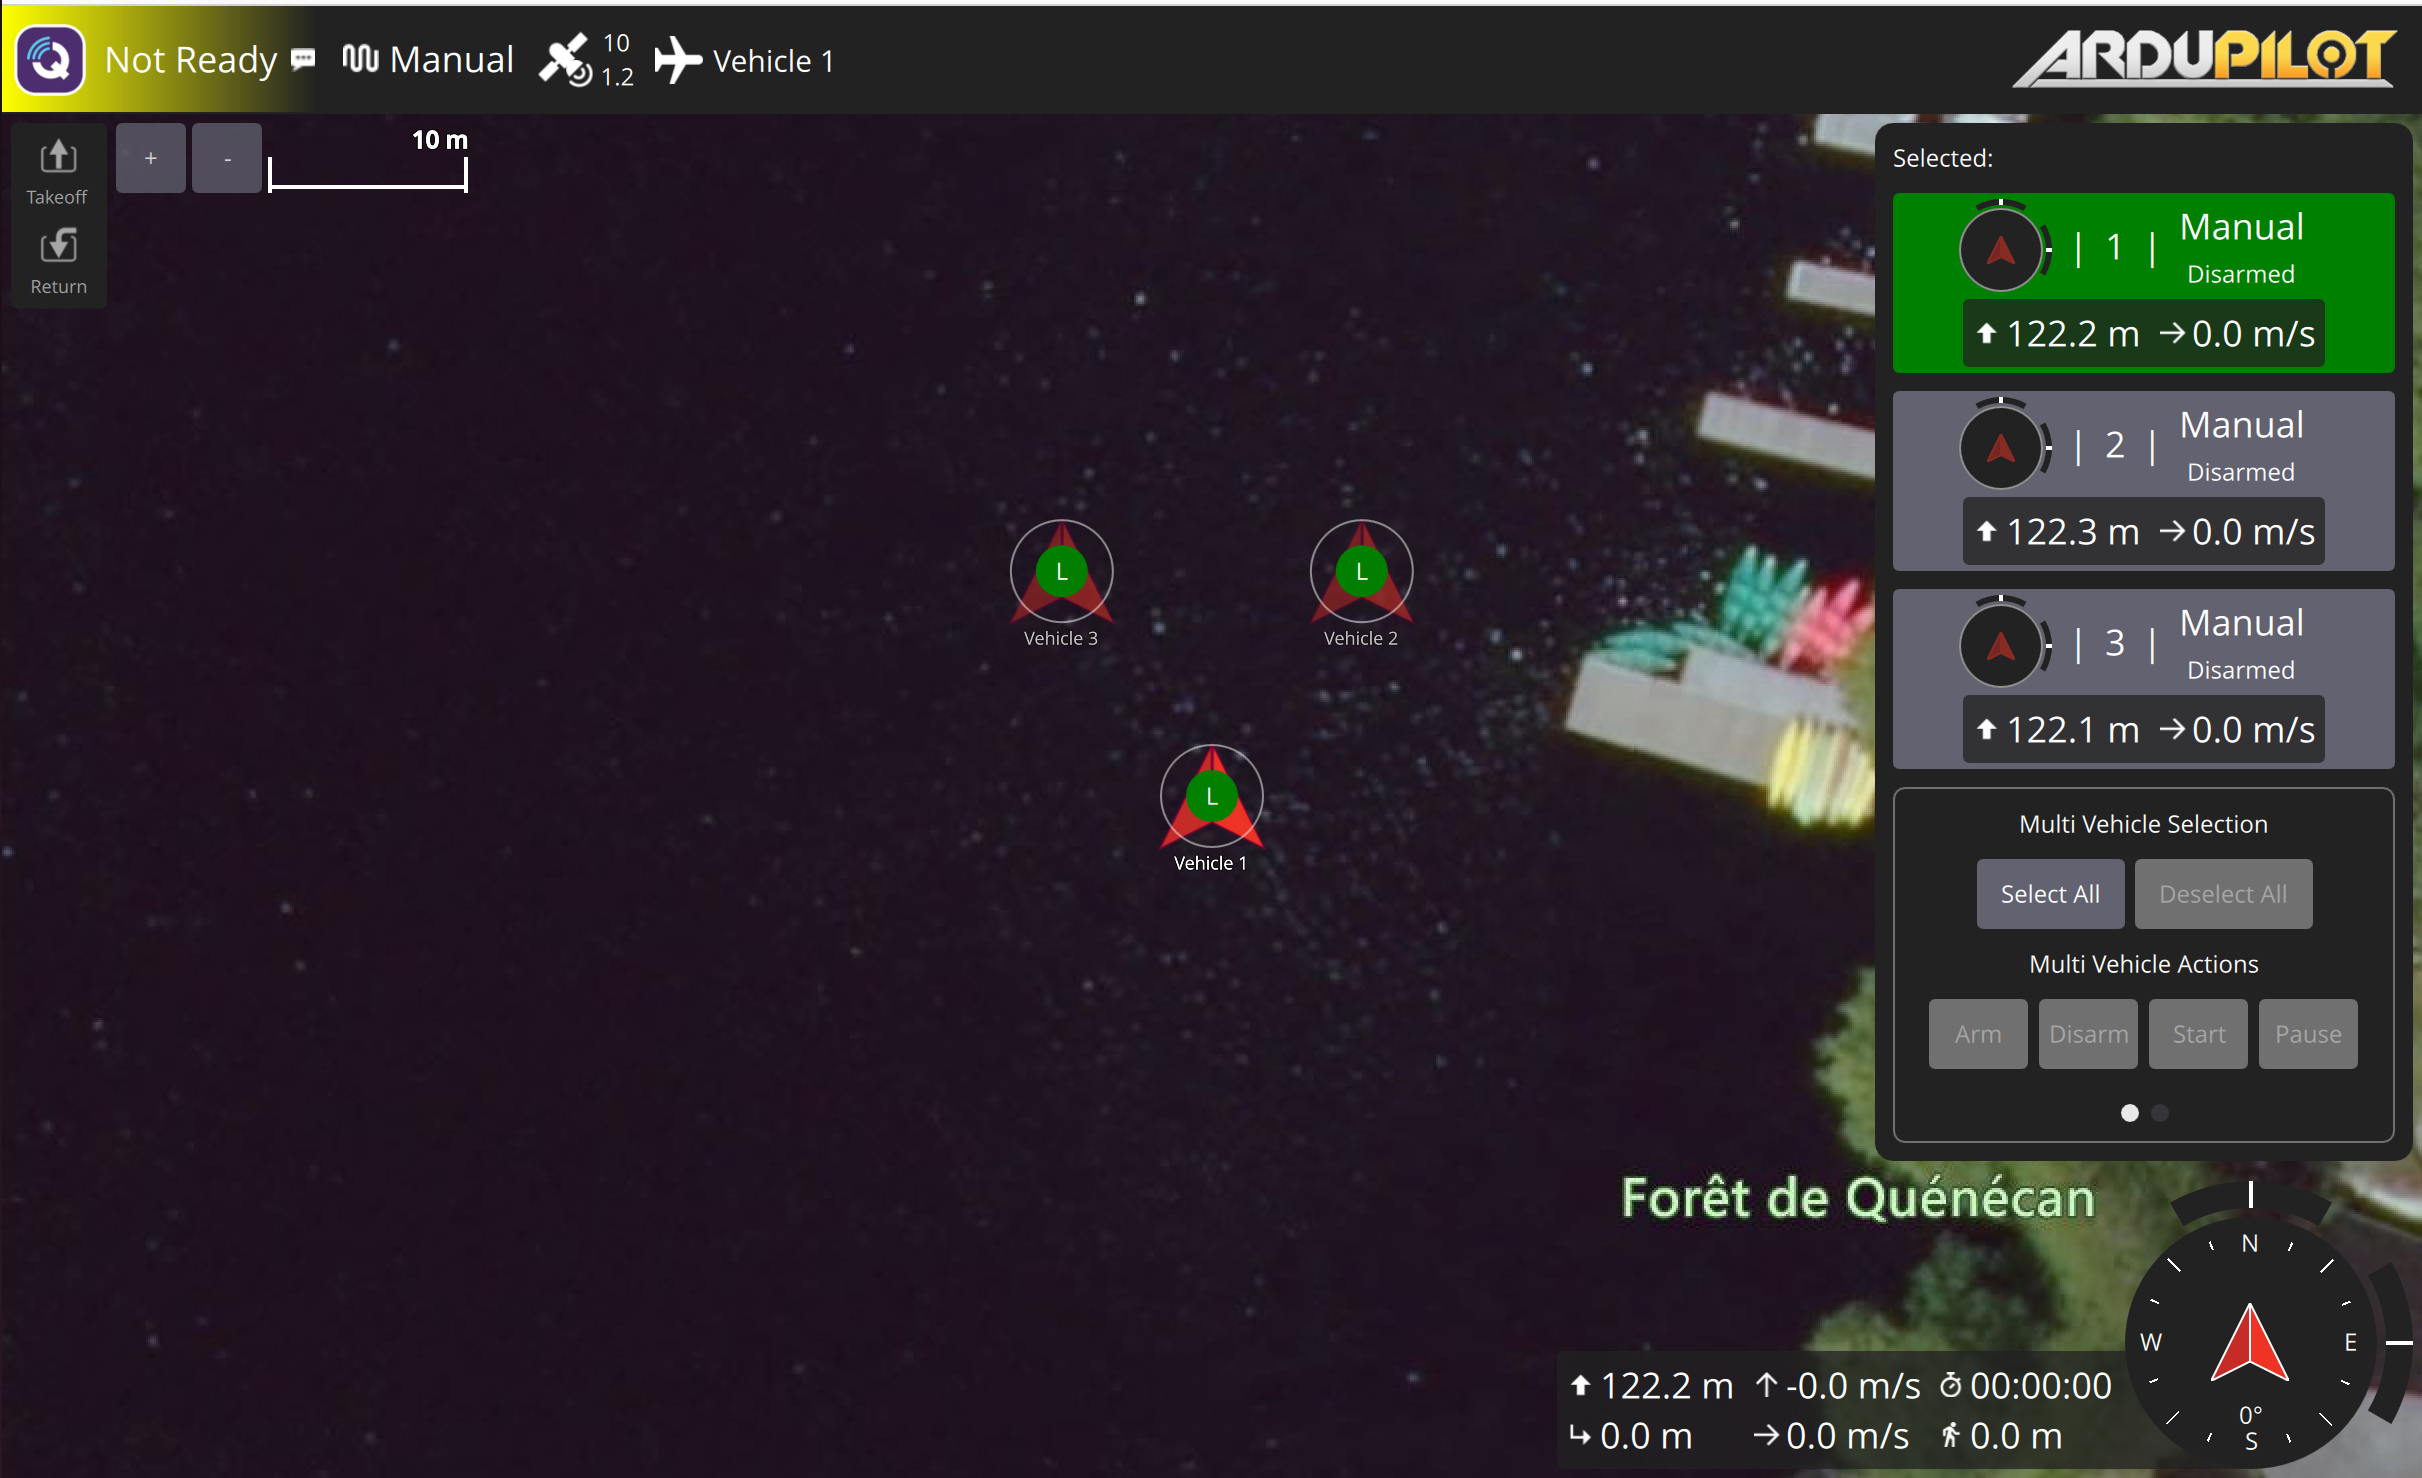
\includegraphics[width=0.5\linewidth]{images/simuQGC.png}
        \caption{Simulation de 3 BlueBoats sur QGC}
        \label{fig:simu_QGC}
    \end{figure}
    
    Malheureusement, bien que les capteurs des robots soient bien légèrement bruité, le mouvement des robots semble idéal. Notamment, imposer une commande de rotation pure au robot le fait bien tourner sur lui même contrairement à ce qui a été observé lors de nos tests réels. De plus, en commandant les robots via MavLink, il semblerait que changer le nombre de robot modifie significativement la commande à envoyer à un robot pour obtenir le comportement voulu. Par exemple, pour une même rotation, un robot seul requérait une commande bien plus élevé qu'un robot d'une simulation en contenant 3. Une explication possible est l'augmentation des temps de calcul nécessaires pour simuler plusieurs robots à chaque fois, puisque cela nécessite ici de lancer pluseurs instances d'Ardupilot. Pour notre utilisation, cette solution présente aussi un autre défaut car QGroundControl ne permet pas de dessiner des figures géométriques sur la carte, et donc ne nous permet pas de visualiser en direct l'estimation de la position des robots par intervalles. Il semblerait que Mission planner le permette, mais ce dernier n'est pas adapté aux systèmes Linux ou MacOS utilisés par les membres de ce groupe et il a donc été décidé de créer notre propre simulation et interface graphique pour communiquer avec les BlueBoats, comme cela sera présenté plus tard dans ce rapport. 